%%% The BEGINNING ~~~~~
%%
% ~ Writes FPG--SI | By Filipe G. VIEIRA & George PACHECO

%% Preamble Settings %%

% Defines document class and paper size ~
\documentclass[twoside, british, a4paper]{article}
\usepackage[paper=portrait, pagesize]{typearea}

\usepackage{amsmath}
\usepackage{amsfonts}
\usepackage{amssymb,upref}
\usepackage{tgheros}
\usepackage{tgtermes}
\usepackage{anyfontsize}
\usepackage{enumitem}
\usepackage{subfig}
\usepackage{siunitx}
\usepackage{balance}
\usepackage{float}

% Fixes margins ~
\usepackage{geometry}
\geometry{reset,ignoreall,
  textheight = 253mm,
  textwidth = 175mm,
  bottom = 21mm,
  inner = 17.5mm,
  footskip = 8mm,
  headsep = 5mm,
  headheight = 10pt}
\usepackage[english]{babel}
\usepackage[utf8]{inputenc}
\usepackage{fancyhdr}
\renewcommand{\headrule}{}
\renewcommand{\footrule}{}

\setlength{\skip\footins}{1.75pc plus 5pt minus 2pt}
\def\footnoterule{
\kern-3mm \hrule height .5pt \kern -.4pt 
\kern 1mm}

\pagestyle{fancy}
\fancyhead[L]{Feral Pigeon Genomics}
\fancyhead[R]{Pacheco et al. 2021}
\fancypagestyle{firstpage}{%
\fancyhf{}
\lhead{}
\rhead{}}

% Loads packages for images ~
\usepackage{graphicx}
\usepackage{rotating}

% Loads packages for comments ~
\usepackage{verbatim}
\usepackage[hang, flushmargin]{footmisc}

% Loads packages for tables ~
\usepackage{float}
\usepackage{multirow}
\usepackage{lmodern}
\usepackage{textcomp}
\usepackage[utf8]{inputenc}
\usepackage[TU]{fontenc}

% Listing of source code ~
\usepackage{listings}
\usepackage{color}
\definecolor{dkgreen}{rgb}{0,0.6,0}
\definecolor{gray}{rgb}{0.5,0.5,0.5}
\definecolor{mauve}{rgb}{0.58,0,0.82}
\lstset{
  frame = tb,
  language = sh,
  aboveskip = 3mm,
  belowskip = 3mm,
  showstringspaces = false,
  columns = flexible,
  basicstyle = {\small\ttfamily},
  numbers = none,
  numberstyle = \tiny\color{gray},
  keywordstyle = \color{blue},
  commentstyle = \color{dkgreen},
  stringstyle = \color{mauve},
  breaklines = true,
  breakatwhitespace = true,
  tabsize = 3}
  
% Changes caption starting text ~
\renewcommand{\figurename}{Supplementary Figure}
\renewcommand{\tablename}{Supplementary Table}

% Loads packages for typing ~
\usepackage{lettrine}
\pdfmapfile{=montserrat.map} 
\renewcommand{\LettrineFont}{
  \fontfamily{iwonal}\fontsize{30}{30}\selectfont
  \color[rgb]{0.25,0.25,0.25}}
\usepackage{marvosym}

\newcommand\myhline{%
  \noindent\rule[.5pt]{\linewidth}{.4pt}\par%
}

\newcommand{\myheaders}[1] {\noindent{\normalsize{\fontfamily{bch}\selectfont{\textbf{#1}}}}}
\newcommand{\mysubheaders}[1] {\noindent{\fontfamily{bch}\selectfont{\textbf{#1}}}}
\newcommand{\mytext}[1] {\noindent{\fontfamily{bch}\selectfont{#1}}}
\newcommand{\mycaptions}[1] {\noindent{\scriptsize{\fontfamily{bch}\selectfont{#1}}}}

% Figure captions
\usepackage{caption}
\DeclareCaptionFont{cfs}{\fontsize{8.5}{10.25}\selectfont}
\DeclareCaptionLabelSeparator{vline}{\;|\;}
\captionsetup{
 labelsep=vline, 
 font={sf,cfs}, 
 labelfont={cfs,bf},
 belowskip=-12pt}
\newcommand{\figurecaption}[2]{\caption[#1]{\textbf{#1.} #2}}
\usepackage{hyperref}
\usepackage[dvipsnames]{xcolor}
\definecolor{mycolor}{HTML}{F7F8E0}
\definecolor{myorange}{RGB}{245,156,74}
\hypersetup{
  colorlinks=true,
  urlcolor=-myorange}

\usepackage{fontawesome}

\usepackage[nopar]{lipsum}
\newcommand\blfootnote[1]{%
  \begingroup
  \renewcommand\thefootnote{}\footnote{#1}%
  \addtocounter{footnote}{-1}%
  \endgroup}

% Loads packages for bibliography ~
\usepackage[
backend = biber,
style = nature,
sorting = ynt
]{biblatex}
\addbibresource{FPGP--MainText.bib}

\usepackage{blindtext}
\usepackage{multicol}

%% Starts Document %%

% Starts document ~
\begin{document}\thispagestyle{empty}

\hfill\break

% Sets title ~
\Large{\bfseries{\fontfamily{cmr}\color[rgb]{0,0,0}\noindent{SUPPLEMENTARY INFORMATION FOR}}} \\

\hfill
\hfill

% Sets title ~
\LARGE{\bfseries{\fontfamily{cmr}\color[rgb]{0.25,0.25,0.25}\noindent{On the Origin and Spread of Feral Pigeons}}} \\

% Sets authorship ~
\fontfamily{cmr} \small \noindent 
George Pacheco\,$^{1}$\textsuperscript{\faEnvelopeO},
Filipe G. Vieira\,$^{1}$,
Michael D. Martin\,$^{1}$,
Morten Tange Olsen\,$^{1}$,
Pavel Hulva\,$^{1}$,
Tânia de Freitas Raso\,$^{1}$,
Peter Njoroge\,$^{1}$,
Concepción Salaberria\,$^{1}$,
Isabel López-Rull\,$^{1}$,
Carles Lalueza-Fox\,$^{1}$,
Oscar Ramírez\,$^{1}$,
María C. Ávila-Arcos\,$^{1}$,
Patricia Rosas Escobar\,$^{1}$,
Rui Faria\,$^{1}$,
Miguel Carneiro\,$^{1}$,
Graciela Sotelo\,$^{1}$,
Jóhannis Danielsen\,$^{1}$,
Nizar Haddad\,$^{1}$,
Fares Khoury\,$^{1}$,
Roi Dor\,$^{1}$,
Ali Halajian\,$^{1}$,
María Belén Arias\,$^{1}$,
Oliver Krone\,$^{1}$,
Susanne Auls\,$^{1}$,
Sampath S. Seneviratne\,$^{1}$,
Kajanka Mathiaparanam\,$^{1}$,
Michael Bunce\,$^{1}$,
Megan L. Coghlan\,$^{1}$,
Jon Fjeldså\,$^{1}$ \&
M. Thomas P. Gilbert\,$^{1}$\textsuperscript{\faEnvelopeO} \\
\myhline

% Sets affiliations ~
\blfootnote{\scriptsize{\fontfamily{cmr}$^1$Section for Evolutionary Genomics, The GLOBE Institute, Faculty of Health and Medical Sciences, University of Copenhagen, Copenhagen, Denmark. $^1$Natural History Museum of Denmark, University of Copenhagen, Øster Voldgade 5–7, 1350 Copenhagen, Denmark. $^1$NTNU University Museum, Norwegian University of Science and Technology, Trondheim, Norway $^1$Department of Zoology, Charles University, Prague, Czech Republic. $^1$Departamento de Patologia, Faculdade de Medicina Veterinária e Zootecnia, Universidade de São Paulo, São Paulo, Brazil. $^1$Ornithology Section, Department of Zoology, National Museums of Kenya, Nairobi, Kenya. $^1$Centro de Investigación en Ecosistemas, Universidad Nacional Autonoma de Mexico, Michoacan, Mexico. $^1$Departamento de Ecología Evolutiva, Museo Nacional de Ciencias Naturales, Madrid, Spain. $^1$Avian Evolution Node, Department of Zoology and Environment Sciences, University of Colombo, Colombo, Sri Lanka. $^1$Institute of Evolutionary Biology, Universitat Pompeu Fabra, Barcelona, Spain. $^1$Department of Animal and Plant Sciences, University of Sheffield, Sheffield, UK. $^1$Centro de Investigação em Biodiversidade e Recursos Genéticos, Universidade do Porto, Vairão, Portugal. $^1$Institute of Evolutionary Biology, Department of Experimental and Health Sciences, University, Pompeu Fabra, Spain. $^1$Departamento de Biologia, Faculdade de Ciências, Universidade do Porto, Porto, Portugal. $^1$University of the Faroe Islands, Tórshavn, Faroe Islands. $^1$National Center for Agricultural Research and Extension, Al-Baqah, Jordan. $^1$Department of Biology and Biotechnology, American University of Madaba, Madaba, Jordan. $^1$Department of Zoology, Tel Aviv University, Tel Aviv, Israel. $^1$Natural History Museum, Imperial College of London, London, United Kingdom. $^1$Department of Biodiversity, Turfloop Campus, University of Limpopo, Polokwane, South Africa. $^1$Department of Wildlife Diseases, Leibniz Institute for Zoo and Wildlife Research, Berlin, Germany. $^1$Vetgenomics SL, Edifici Eureka, Campus UAB, Barcelona, Spain. $^1$Trace and Environmental DNA (TrEnD) Laboratory, Department of Environment and Agriculture, Curtin University, Perth, Australia.\\ \textsuperscript{\faEnvelopeO}Correspondence should be addressed to \href{mailto:ganpa@aqua.dtu.dk}{ganpa@aqua.dtu.dk} (G.P.) \& \href{mailto:tgilbert@sund.ku.dk}{tgilbert@sund.ku.dk} (M.T.P.G.)}}

\hfill

% Suplementary Notes %

\begin{multicols}{2}
\myheaders{Suplementary Notes} \\
\mysubheaders{Sampling effort.} \mytext{To investigate the genomic patterns of current pigeon populations of different evolutionary histories, we intentionally targeted our sampling to cover four distinct categories (Figure 1). Furthermore, to help root the evolutionary relationships between these groups, we also included a small number of individuals representing the Columba livia intermedia (Strickland, 1844) subspecies. Specifically in this regard, we sampled five populations from Sri Lanka, where two of them were from urban localities (Colombo and Trincomalee), one was from a Conservation National Park (Pigeon Island) and two others were captive populations maintained by local breeders (Wattala and Wellawatte) (Supplementary Fig. 1). To check for data reproducibility, we sequenced two of the samples twice (Tehran\textunderscore16-GBS and Perth\textunderscore02-GBS) to serve as replicates. Finally, to serve as external outgroups, we also generated data from five samples of (\textit{Columba palumbus Linnaeus}, 1758) captured in Copenhagen (Denmark), one captive sample of (\textit{Streptopelia risoria} Linnaeus, 1758), and additionally incorporated previously published whole genome resequence data from a Columba rupestris8. (we also included the WGS library to serve as another replicate) (Supplementary Spreadsheet).}

% Methods %
\myheaders{Methods} \\

\end{multicols}

\newpage
\clearpage

\begin{multicols}{2}
\myheaders{References}
\printbibliography[heading=none]

\hfill

\end{multicols}

\newpage
\clearpage

\begin{figure}[ht]
\centering
\includegraphics[width=1\textwidth]{../FPG--Plots/FPG--Stats/FPG--CoverageHeatMap/FPG--CoverageHeatMap.pdf}
\caption*{\mycaptions{\textbf{Supplementary Fig. 1. Coverage heatmap.} Heatmap based on the presence/absence matrix. Individual samples are represented by each column, whereas clusters of loci are represented by the rows.}}
\label{SI:FPG--CovHeatMap}
\end{figure}

\hfill

\begin{figure}[H]
\centering
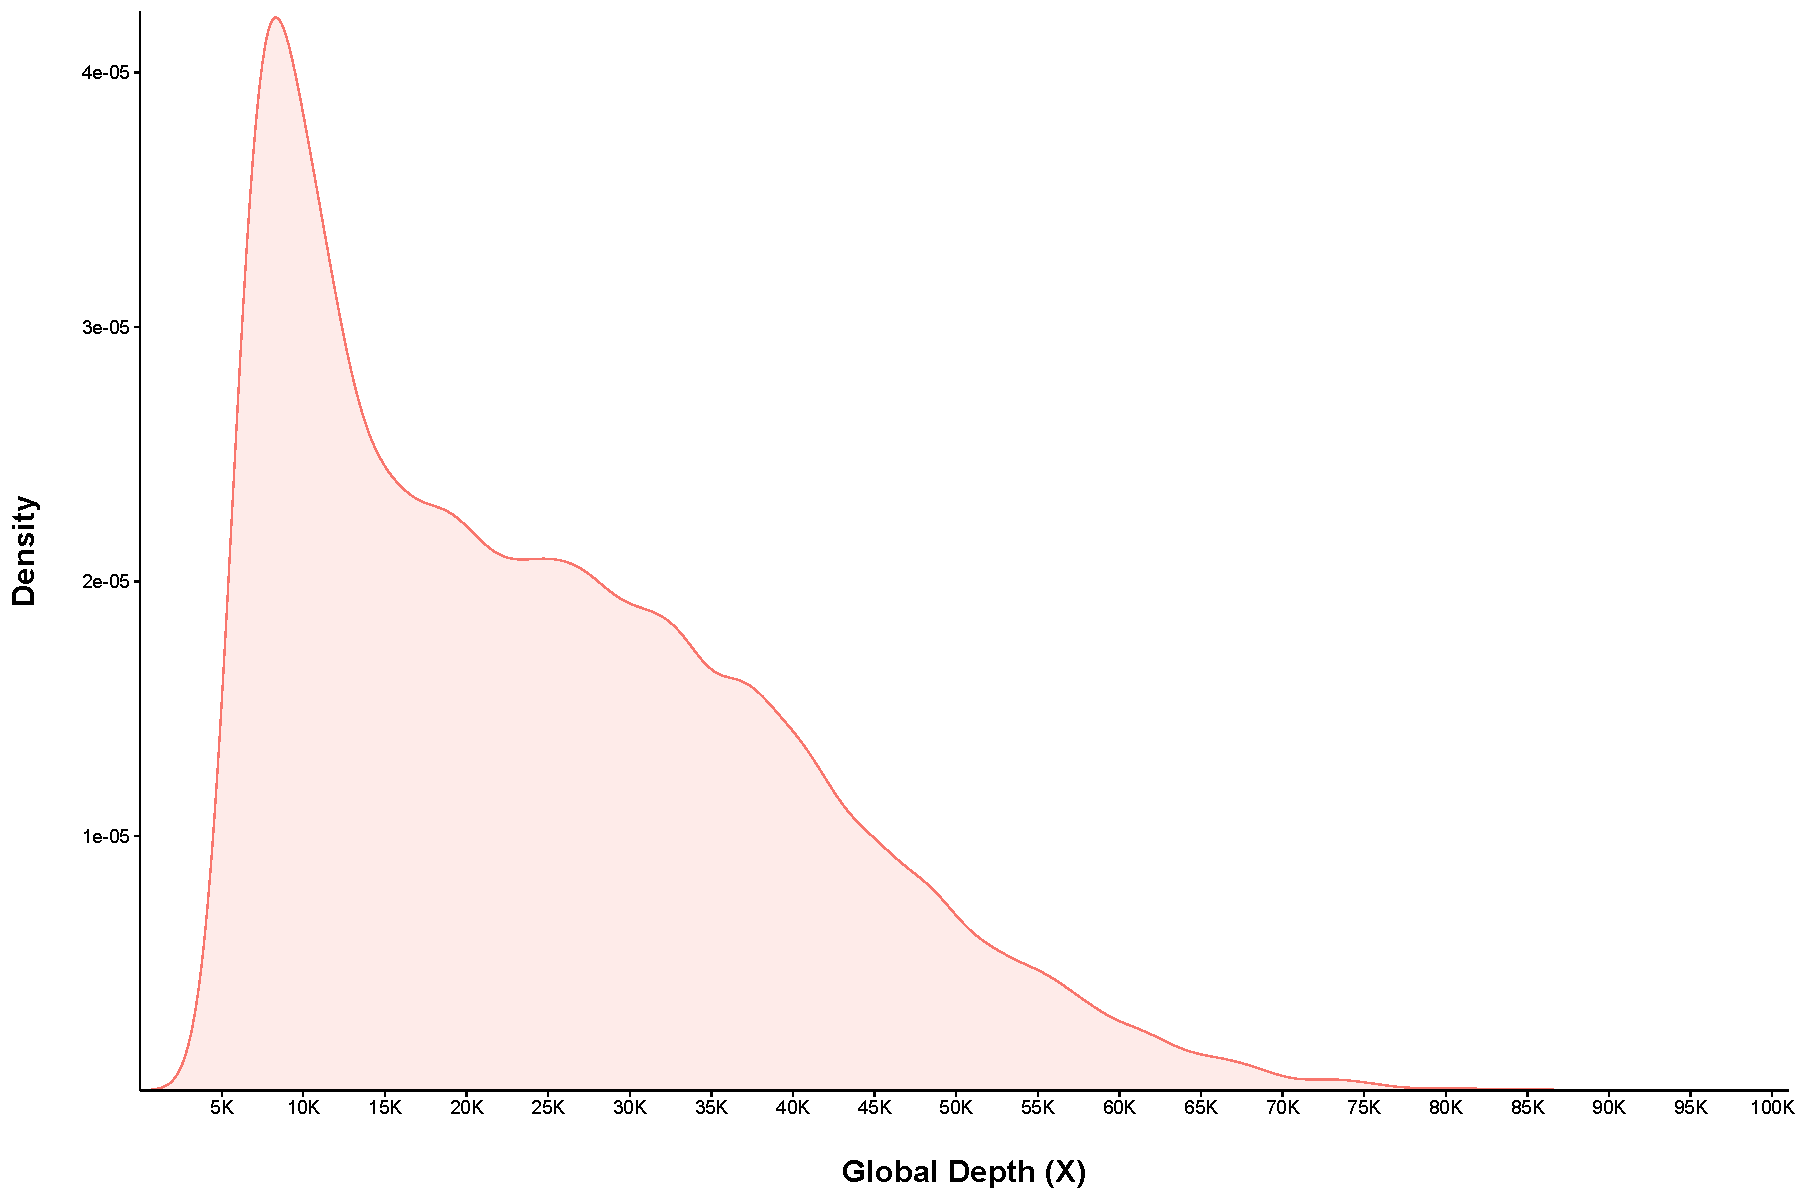
\includegraphics[width=1\textwidth]{../FPG--Plots/FPG--Stats/FPG--GlobalCoverage/FPG--GlobalCoverage.pdf}
\caption*{\mycaptions{\textbf{Supplementary Fig. 1. Global depth distribution.} Heatmap based on the presence/absence matrix. Individual samples are represented by each column, whereas clusters of loci are represented by the rows.}}
\label{SI:FPG--CovDistribution}
\end{figure}

\begin{figure}[!ht]
\centering
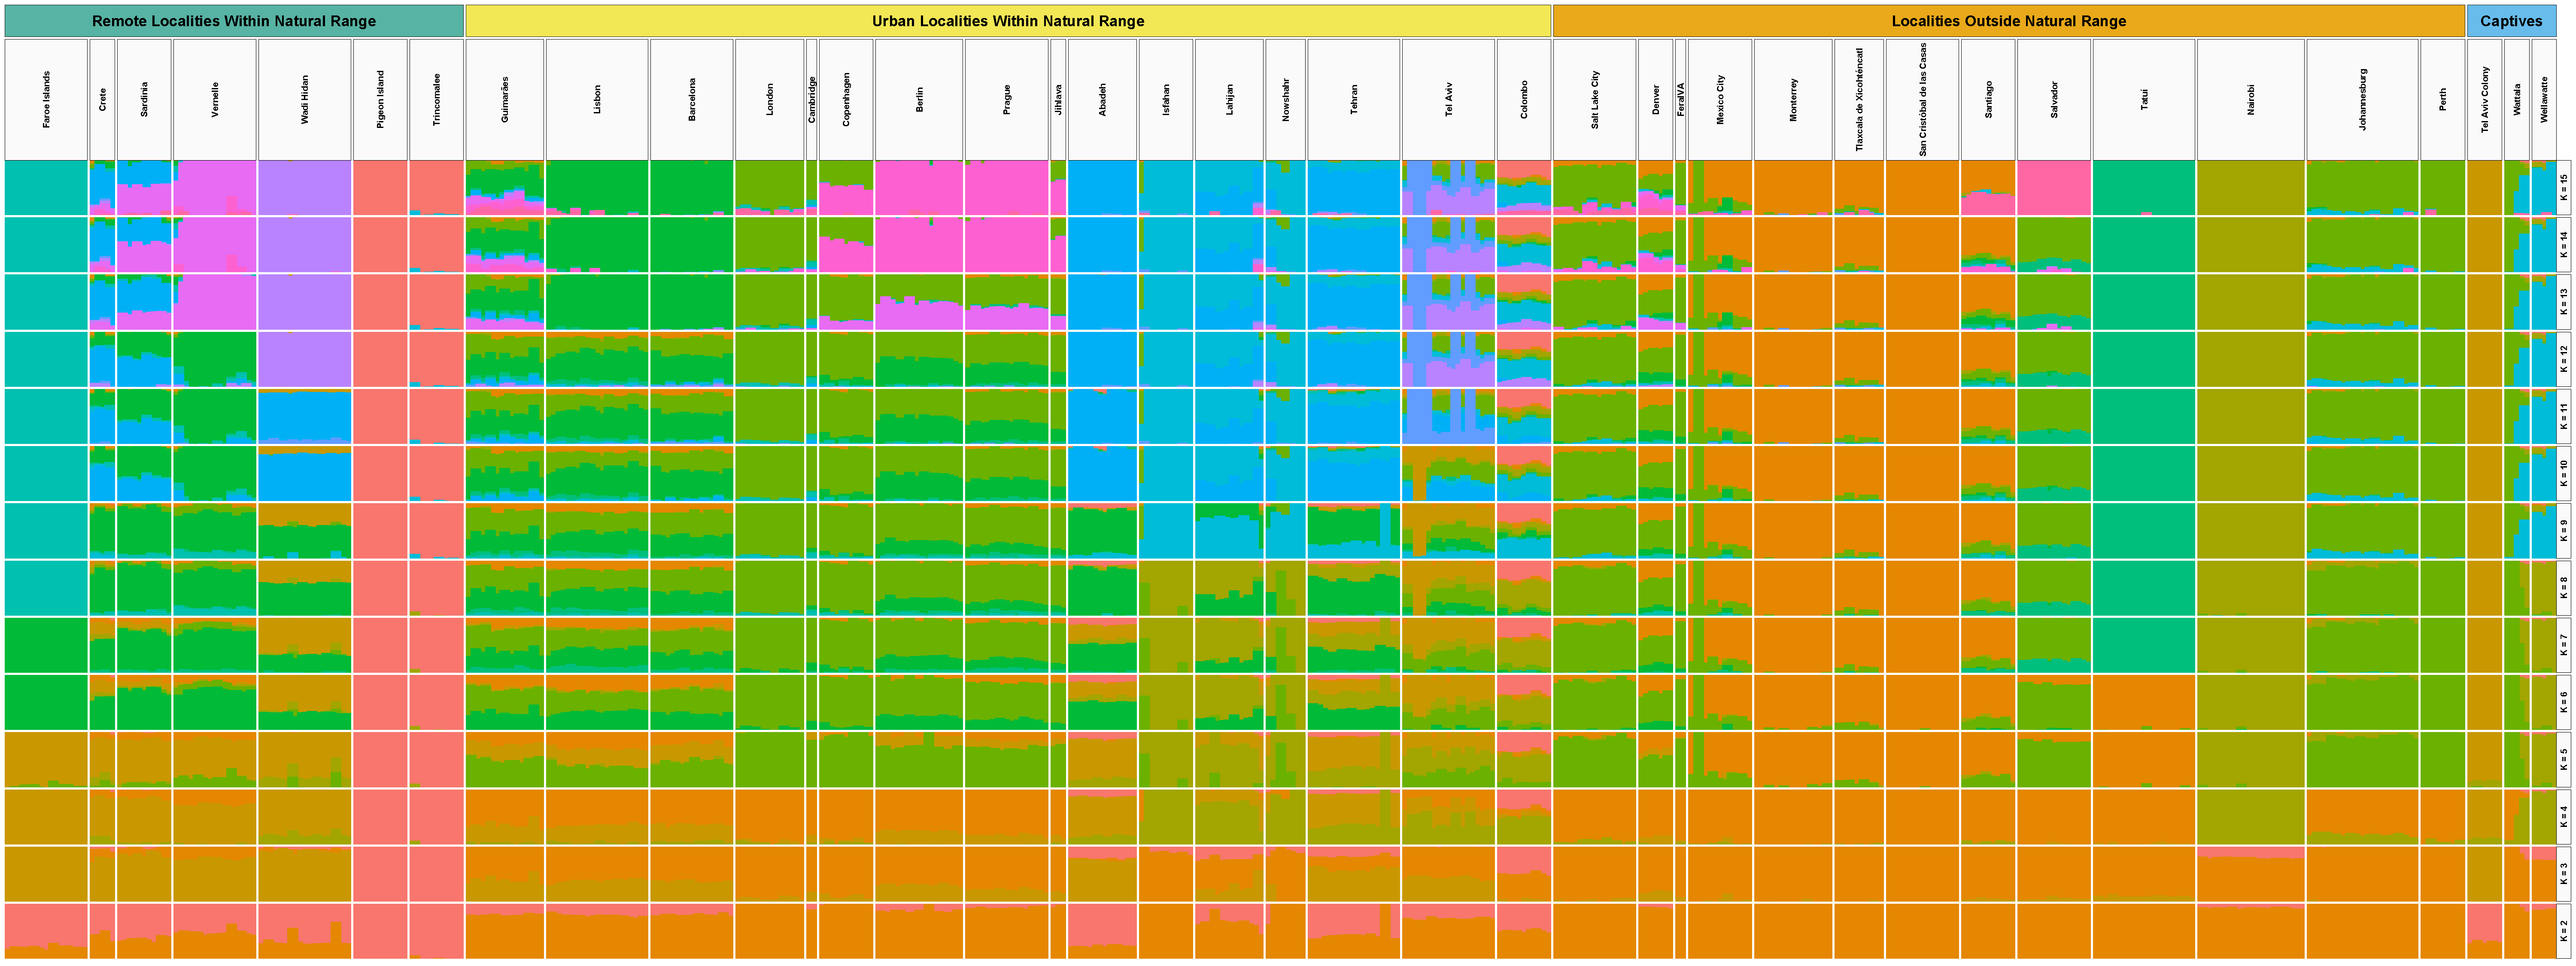
\includegraphics[width=1\textwidth]{../FPG--Plots/FPG--ngsAdmix/FPG--ngsAdmix_Labels-RColours.pdf}
\caption*{\mycaptions{\textbf{Fig. 3 Estimation of Admixture proportions.} Individuals are represented by columns, while rows depict the Admixture proportions based on the assumption of different numbers of ancestral populations (K = 2 - 15). Individuals are sorted by sampling locality (light grey upper labels) and grouped per biological status}}
\label{MainText:FPG--ngsAdmixSI}
\end{figure}
  
\begin{figure}[!ht]
\centering
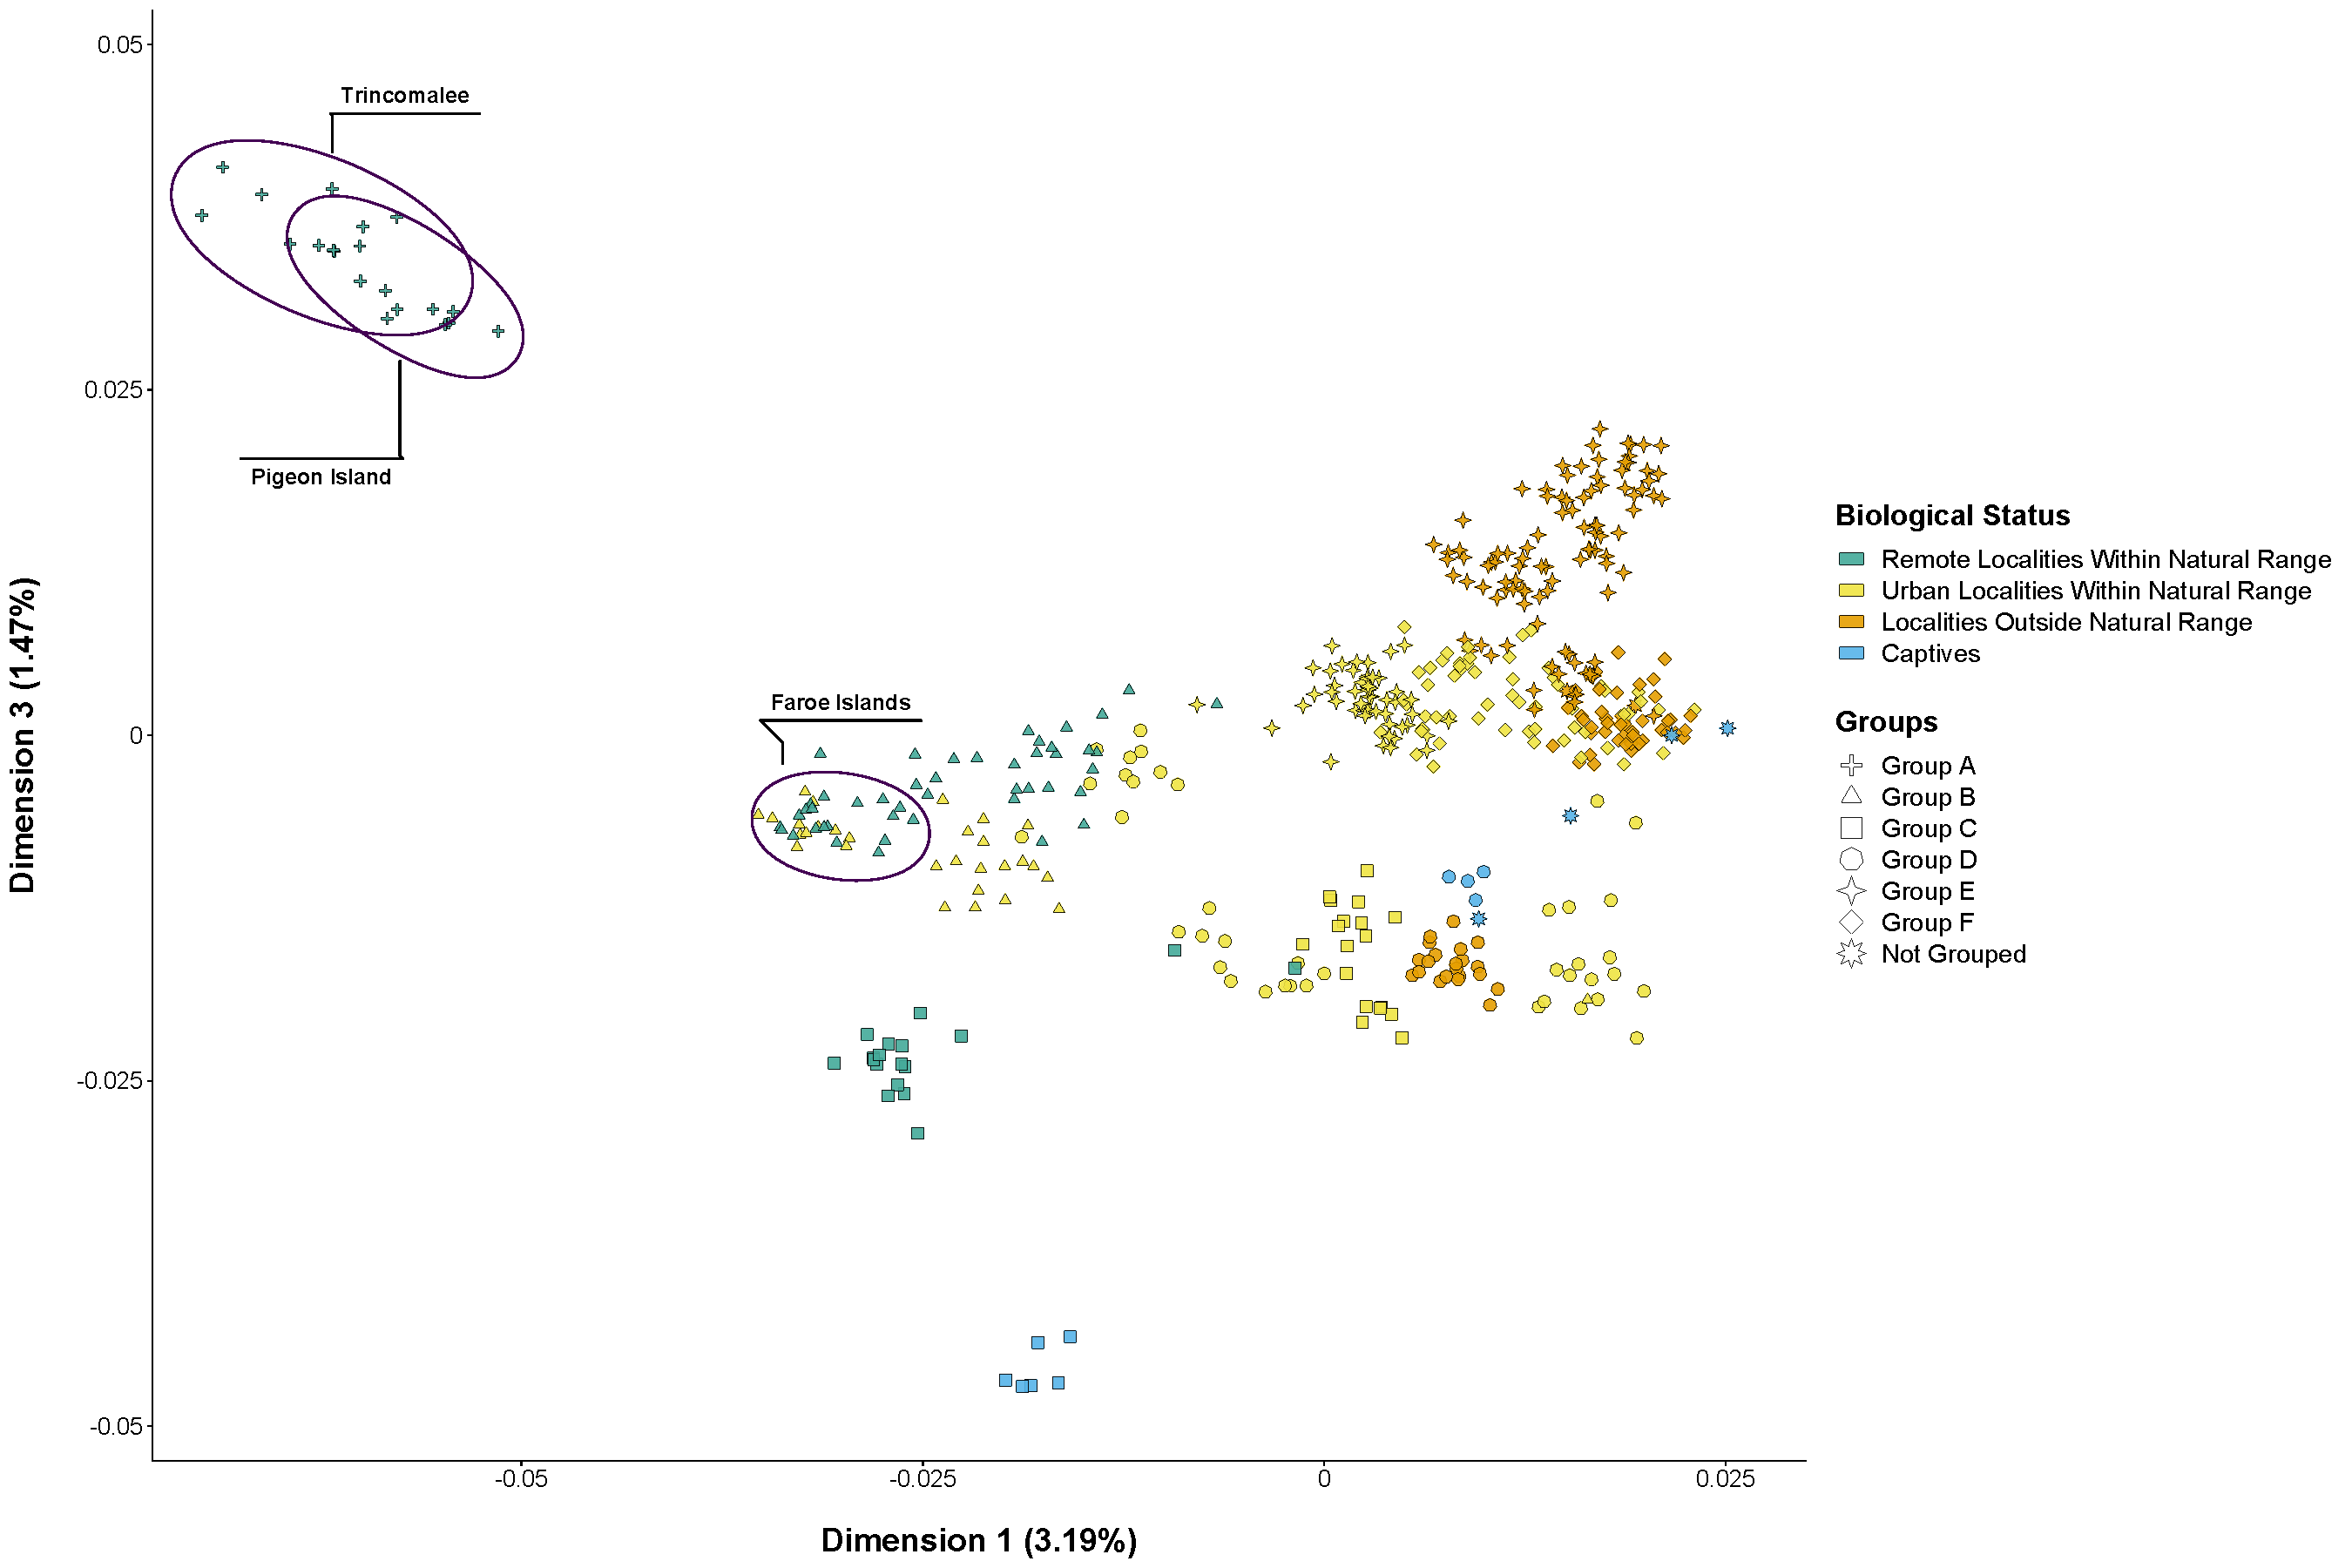
\includegraphics[width=1\textwidth]{../FPG--Plots/FPG--MDS/FPG--MDS_13.pdf}
\caption*{\mycaptions{\textbf{Fig. 2 Multidimensional scaling analysis.} a) Dimensions 1 and 3 are plotted. b) Dimensions 2 and 3 are plotted. Each point on the plot represents a single individual. The ellipses represent the rough distribution of the two most distinct groups.}}
\label{MainText:FPG--MDS_13}
\end{figure}

\end{document}

% 
%%
%%% The END ~~~~~